\documentclass[12pt]{article}

\usepackage{amsmath}
\usepackage{graphicx}
\usepackage{hyperref}
\usepackage{cite}
\usepackage[margin=1.2in]{geometry}

\providecommand{\eqn}[1]{eqn.~(\ref{eqn:#1})}
\providecommand{\tab}[1]{Table~\ref{tab:#1}}
\providecommand{\fig}[1]{Figure~\ref{fig:#1}}

\providecommand{\vecsymbol}[1]{\ensuremath{\boldsymbol{#1}}}
%\providecommand{\pv}{\vecsymbol{p}}
%\providecommand{\deltav}{\vecsymbol{\delta}}

\title{Observing Hour Angle Assignments\\
for the DESI Survey\\
\vspace{5mm}{\large\bf DESI-doc-3060-v1}}
\author{David Kirkby, Kyle Dawson}

\begin{document}
\maketitle

\section{Introduction}

This note briefly describes the algorithm used to assign a near-optimal observing hour angle (HA) to each tile in the DESI footprint~\cite{desi-717} and documents the result for the current baseline survey strategy~\cite{desi-1767, desi-1770}. The algorithm is implemented in python code in the {\tt desisurvey} package\footnote{\url{https://github.com/desihub/desisurvey}} and the reader is referred there for implementation details. A jupyter notebook to create the plots in this note is provided under {\tt desisurvey/doc/nb/}.

\section{Algorithm Description}

The algorithm is run separately for each program (DARK, GRAY, BRIGHT) and has two main inputs:
\begin{itemize}
    \item the date range to optimize the program for, and
    \item a list of tiles remaining to observe in the program.
\end{itemize}
The date range determines the available hours at each apparent local sidereal time (LST) for the specified program, taking into account planned shutdowns (during the annual monsoon and full-moon), expected weather outages each month, and the solar and lunar ephemerides that determine the time available to the program during each night. The list of tiles determines the required exposure time at each LST, given HA assignments and an exposure-time calculator.

The basic idea of the algorithm is to iteratively adjust the HA assignments of each tile to minimize a score function that accounts for two metrics:
\begin{itemize}
    \item the matching of available and planned LST usage, and
    \item the total required exposure time.
\end{itemize}
We run the algorithm in two different modes:
\begin{itemize}
    \item Start of survey: optimize all tiles over the nominal five-year survey dates.
    \item Afternoon planning: optimize all tiles not yet observed for the remainder of the survey.
\end{itemize}
The first mode is only used before the survey starts and then only needs to be rerun after a change in the definition of the tiles, programs, or nominal observing schedule. The second mode is run regularly during the survey and adjusts HA assignments to reflect actual observing progress and any schedule changes.

Most of the assumptions used in the survey planning and program definitions are listed in a text configuration parameter file\footnote{\url{https://github.com/desihub/desisurvey/blob/master/py/desisurvey/data/config.yaml}}. One parameter, in particular, limits the HA solution space by requiring that all tiles are observed above a minimum altitude angle of $30^\circ$.  In order to allow some leeway for exposure duration, we calculate a maximum $|\text{HA}|$ for each tile corresponding to its declination and a minimum altitude of $35^\circ$.

\subsection{Initialization}

The initial HA assignments that are subsequently optimized can be set in three different ways:
\begin{itemize}
    \item Read HAs from a file.
    \item Set all HAs to zero.
    \item Assign HAs to approximately match the cummulative distribution functions of available and planned LST usage.
\end{itemize}
The first method is used during afternoon planning, while the last two methods bootstrap the optimization at the start of the survey.

Assigning zero initial HAs minimizes the total exposure time required, but generally leads to a large mismatch between the available and planned LST usage. While conceptually simple, this approach is inefficient since it requires a large number of iterations to converge to a near-optimal solution. \fig{LST_zero0} compares the available and planned LST usage after initializing
all HAs to zero.

\begin{figure}[htb]
\begin{center}
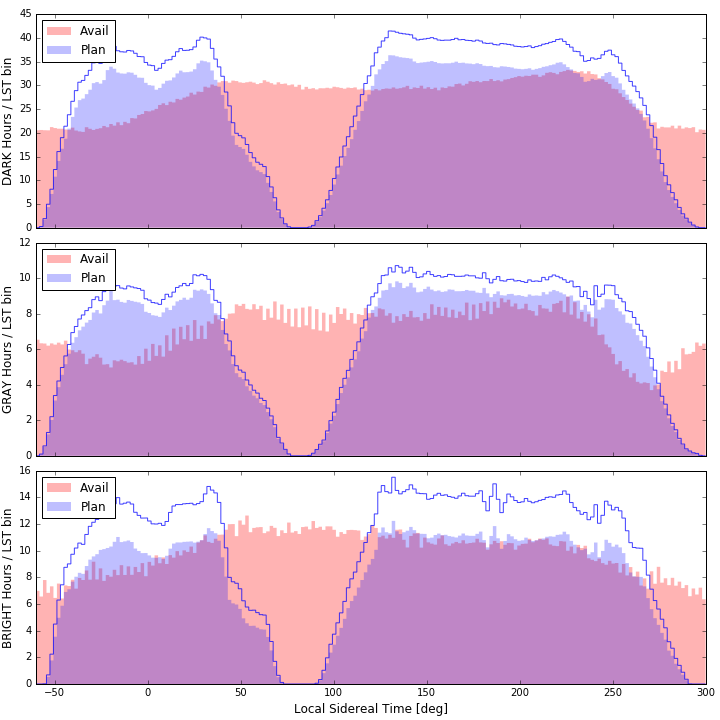
\includegraphics[width=6in]{LST_zero0}
\caption{Available (red) and planned (blue) LST usage for the HA=0 initialization method.  The blue outline histogram shows the planned usage rescaled to the area of the available LST histogram.  The LST axis starts at $-60^\circ$ and the gaps in the planned usage correspond to the breaks between the southern and northern galactic caps in the DESI footprint.}
\label{fig:LST_zero0}
\end{center}
\end{figure}

An alternative bootstrap initialization, which we refer to as the ``flat'' method, is to approximately match the cummulative distribution of available LST to planned LST usage. We first tabulate the available survey time $a_j$ in $n$ LST bins
$$
\theta_j \le \theta < \theta_{j+1} \quad , \quad \theta_j = (j/n) 360^\circ \; ,
$$
where $j$ ranges from $0$ to $n-1$, then calculate its cummulative distribution function (CDF) in $n+1$ steps as
$$
A_0 = 0 \quad , \quad
A_{j+1} = \frac{\sum_{k=0}^{j} a_k}{\sum_{k=0}^{n-1} a_k} \; .
$$
Next, we approximate the CDF of planned LST usage of $i = 0, 1, \ldots, N-1$ tiles with all HAs equal zero as:
$$
P_i = \frac{\sum_{k=0}^{i} \Delta t_k}{\sum_{k=0}^N \Delta t_k} \; ,
$$
where $\Delta t_k$ is the expected exposure time for tile $k$ at HA=0 and tiles are ordered in increasing right ascension (RA). Finally, we match the available and planned CDFs by adjusting each tile's LST $\tilde{\theta}_i$ using linear interpolation of the inverse mapping $A_j \rightarrow \theta_j$ evaluated at each $P_i$.  We then select
$$
\text{HA}_i = \tilde{\theta}_i - \text{RA}_i
$$
as the initial HA for tile $i$.

Since LST and RA are periodic, the initial HAs obtained with this method depend on an arbitrary choice of starting angle, which corresponds to an LST where all tiles will have HA=0. In practice, we repeat this initialization on a grid of possible starting angles and select the one with the minimum score function (defined below). \fig{LST_flat0} compares the available and planned LST usage after initializing all HAs with this method. \fig{HA_flat0} shows the distribution of initial HAs over the sky for each pass of each program.

\begin{figure}[htb]
\begin{center}
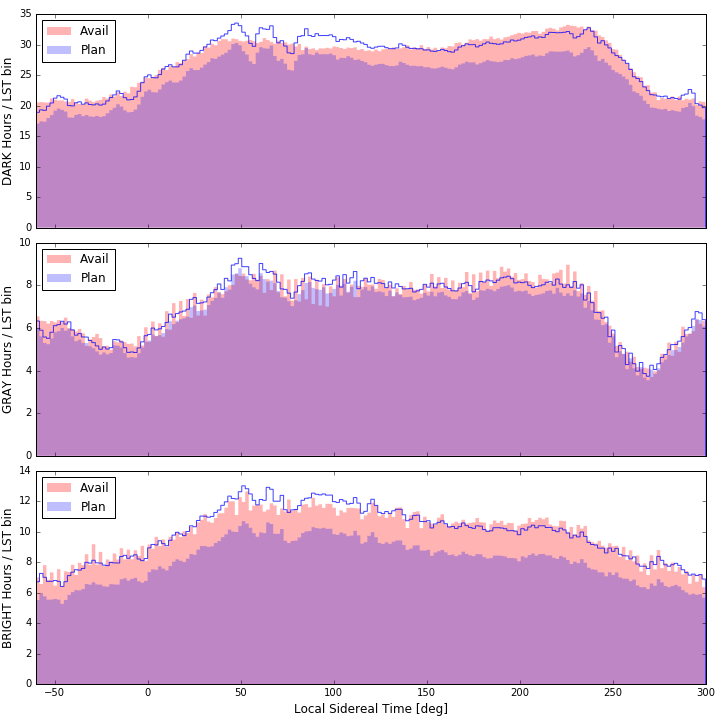
\includegraphics[width=6in]{LST_flat0}
\caption{Available (red) and planned (blue) LST usage for the flat initialization method.  The blue outline histogram shows the planned usage rescaled to the area of the available LST histogram.  The LST axis starts at $-60^\circ$.}
\label{fig:LST_flat0}
\end{center}
\end{figure}

\begin{figure}[htb]
\begin{center}
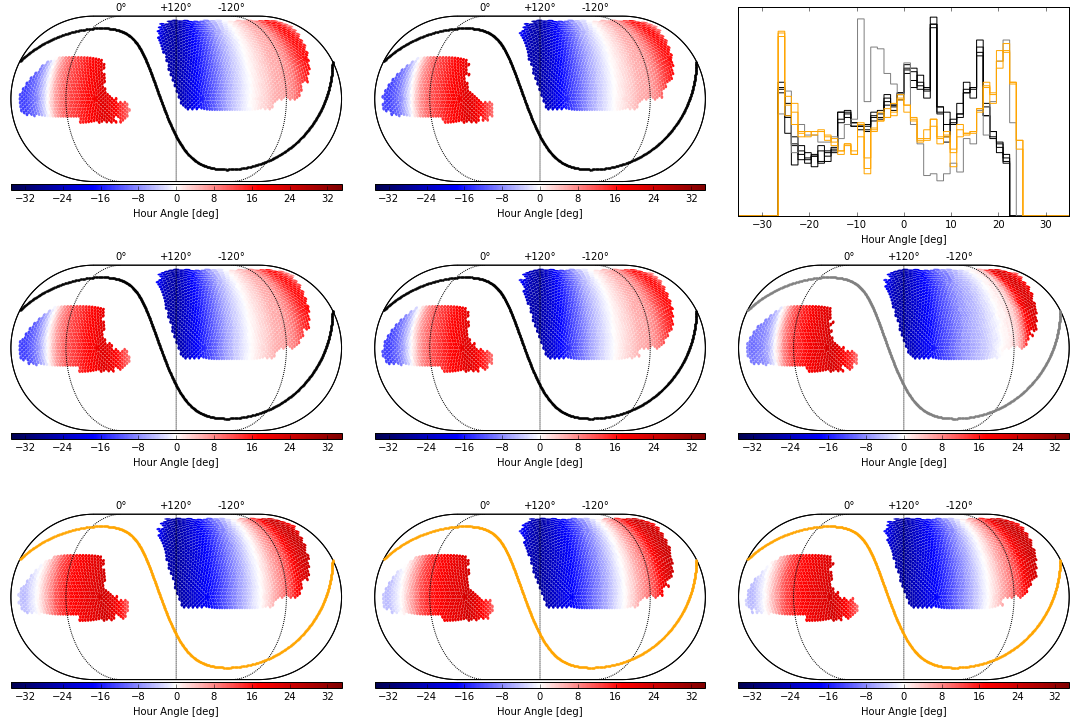
\includegraphics[width=6in]{HA_flat0}
\caption{All-sky maps of the tiles in each pass (0-7) color coded by their initial HA assignment using the ``flat'' initialization method.  Passes 0-1 (top row), 2-4 (middle row) and 5-7 (bottom row) correspond to the DARK (0-3), GRAY (4) and BRIGHT (5-7) programs.  Histograms show the HA distribution in each pass, color coded by the pass program: black (DARK), gray (GRAY) and orange (BRIGHT).}
\label{fig:HA_flat0}
\end{center}
\end{figure}

This CDF-matching ``flat'' method does a good job of matching the available and planned LST usage, but generally increases the total exposure time required more than necessary. The approximations in this method are that:
\begin{itemize}
    \item Exposure times are calculated for HA=0 and then used to estimate non-zero HAs for each tile.
    \item The contribution from each exposure is assumed to contribute at a single LST rather than being spread of LST in proportion to the length of the exposure.
    \item The CDF matching procedure enforces that the ordering of tile LSTs matches the ordering of tile RAs, but this may not be optimal.
\end{itemize}
The iterative improvement scheme described below does not have any of these limitations.

\subsection{Exposure Times}

Exposure times for observing during the DARK program are estimated as:
$$
\Delta t = \Delta t_{\text{nom}}\, f_{\text{dust}}\, f_{\text{airmass}}\,
f_{\text{seeing}}\, f_{\text{transp}} \; ,
$$
where the nominal exposure time $\Delta t_{\text{nom}}$ is specified by the program (1000 seconds for DARK and GRAY, and 300s for BRIGHT) and the remaining dimensionless factors correct for the actual versus nominal observing conditions: dust extinction, airmass, seeing, and atmospheric transparency.

The dust factor is fixed by the median value of $E_{B-V}(\text{RA}, \text{DEC})$ over the tile and given by:
$$
f_{\text{dust}} = 10^{E_{B-V}}
\quad, \quad \alpha = 2.64 \; ,
$$
The airmass factor is a function of the airmass $X(\text{DEC}, \text{RA})$ and given by:
$$
f_{\text{airmass}} = X^{1.25} \; .
$$
The remaining factors will vary stochastically during actual observing so our goal here is simply to account for their mean time-integrated effect using the formalism described below.

Suppose the instantaneous signal-to-noise ratio depends on an observing parameter $x$ according to
$$
\frac{d\nu}{dt}(x) = f(x)^{-1}
$$
then under nominal constant conditions $x(t) = x_0$, the integrated signal-to-noise over a time interval $T$ is:
$$
\nu(T) = \int_0^T f(x(t))^{-1}\, dt =  T / f(x_0) \; .
$$
However, if $x(t)$ varies stochastically with mean $\mu_x$ and variance $\sigma_x^2$, then
\begin{align}
\nu(T) &= \int_0^T f(x(t))^{-1}\, dt \\
&= \int_0^T (1/f)\left(
\mu_x + (x(t) - \mu_x)\right) \\
&\simeq \int_0^T \left[ (1/f)(\mu_x) + (1/f)'(\mu_x) (x - \mu_x)
+ \frac{1}{2} (1/f)''(\mu_x) (x - \mu_x)^2 \right]^{-1} \\
&= \frac{T}{f(\mu_x)}\left[1 + g(\mu_x) \sigma_x^2 \right] \; ,
\end{align}
with
$$
g(x) \equiv \frac{f'(x)^2}{f(x)^2} - \frac{f''(x)}{2 f(x)} \; .
$$
We define the time-integrated exposure time factor $F_x$ as the increase in time relative to nominal conditions required to achieve the same integrated signal to noise $\nu(T)$, i.e.
$$
\nu(F_x T) = T f(x_0) \; .
$$
We can then evaluate $F_x$ approximately using:
$$
F_x \simeq \frac{f(\mu_x)}{f(x_0)} \left[1 +
g(\mu_x) \sigma_x^2 \right]^{-1} \; .
$$

Consider the effects of transparency, with
$$
f(x) = 1/x \; ,
$$
and seeing, with
$$
f(x) = a + b x + c x^2 \quad , \quad (a,b,c) = (4.6, -1.55, 1.15) \; .
$$
\tab{expfac} below summarizes the expected time-integrated exposure factors using means and variances obtained from a weather simulated based on empirical distibutions. We see that the second-order corrections increase the seeing exposure factor by about 7\% but have no effect on the transparency. Assuming that transparency and seeing are uncorrelated, we expect an overall factor of 1.27 during the DARK program.

\begin{table}[htb]
\begin{center}
\begin{tabular}{lccccc}
Condition & Median & $\mu_x$ & $\sigma_x$ & $g(\mu_x)$ & $F_x$ \\
\hline
Seeing & $1.19$" & $1.41$" & $0.76$" & -0.113 & 1.175 \\
Transparency & $1.00$ & $0.93$ & $0.00$ & 0.000 & 1.078 \\
\hline
\end{tabular}
\caption{Summary of simulated weather study to establish the time-integrated exposure factors due to variable seeing and transparency.}
\label{tab:expfac}
\end{center}
\end{table}

Exposure times during the GRAY and BRIGHT programs have an additional factor due to scattered moonlight, but further study is needed to accurately estimate its impact.  We therefore assign average exposure time factors to account for seeing, transparency and moon of: 1.3 (DARK), ?? (GRAY) and ?? (BRIGHT).

\subsection{Iteration}

For details on the iteration scheme, refer to the {\tt optimize.Optimizer.improve} method of the {\tt desisurvey} package. Here we just provide a high-level sketch of the algorithm.

Each iteration is governed by an HA adjustment size parameter, $\delta\text{HA}$, which we gradually decrease in an outer loop as described in the next section. Given an adjustment size, we select a single tile to adjust then recompute the planned LST usage using its new HA and exposure time (due to its change of airmass with HA). The total number of iterations (single-tile adjustments) required to obtain near-optimal HA assignments starting from HA=0 is typically 20--30 times the total number of tiles. The algorithm has several stochastic elements in order to avoid getting stuck in a local minimum, but uses a single source of pseudo-random numbers to ensure reproducibility.

The score function that each iteration attempts to improve combines two figures of merit which we refer to as RSME and LOSS.

RMSE measures the fractional deviation between the available ($A_i$) and planned ($P_i$) LST usage histograms using
$$
\text{RMSE} \equiv \frac{1}{\sum_i^n P_i}
\left( n \sum_i^n (s A_i - P_i)^2 \right)^{1/2}
$$
where the scale factor
$$
s = (\sum_i^n P_i) / (\sum_i^n A_i)
$$
normalizes the total available LST to the total planned usage so that RMSE measures deviations in shape only.  LOSS compares the total exposure time required with the current plan ($T_P$) with the minimum possible total time ($T_0$) when all tiles are observed with HA=0, using
$$
\text{LOSS} \equiv (T_P - T_0) / T_0 \; .
$$
After some experimentation, we combine these dimensionless metrics with equal weight,
$$
\text{SCORE} = \text{RMSE} + \text{LOSS} \; ,
$$
so that RMSE typically dominates during the first phase of optimization, then LOSS dominates towards the end.  Typical final values after optimization are RMS $\simeq 1$\% and LOSS $\simeq 3$\%.

We automatically switch between two algorithms to select the set of candidate tiles to adjust during each iteration: a fast algorithm that is typically selected when RMSE dominates the score, and a slower brute-force algorithm that is typically selected when LOSS dominates.  The fast algorithm first identifies which LST bin would maximally improve RMSE when tiles are shifted away from it, and then only considers tiles whose exposures overlap that bin.  The slow algorithm considers a 20\% random subset of all tiles.  We next rank all tiles in the candidate set according to how much they improve the SCORE when adjusted. We usually pick the tile with the best improvement but will sometimes randomly pick a lower-ranked tile. The size of the HA adjustment is randomly generated from a Rayleigh distribution with mean fixed to the input adjustment-size parameter $\delta\text{HA}$.

\subsection{Annealing and Termination}

The {\tt surveyinit} script uses the {\tt optimize.Optimizer} class to coordinate the overall HA assignment task. Optimization proceeds in ``cycles'' of $n$ adjustments with fixed parameters, where $n$ equals the number of tiles to optimize. After each cycle, the distribution of HAs is smoothed over the sky,
$$
\text{HA}_j = (1 - \alpha)\,\text{HA}_j + \alpha\,\overline{\text{HA}}_j
$$
where $\overline{\text{HA}}_j$ is the weighted average of neighboring HAs,
$$
\overline{\text{HA}}_j = \sum_{k\ne j} \omega_{jk}\,\text{HA}_k \; ,
$$
and $\alpha$ controls the amount of smoothing.  Smoothing weights are Gaussian in the separation angle $\theta_{jk}$ between pairs of tiles,
$$
\omega_{jk} = \exp\left( -0.5(\theta_{jk} / \sigma_S)^2 \right) \; ,
$$
with a smoothing length $\sigma_S \simeq 10^\circ$.

After each complete cycle, the adjustment size $\delta\text{HA}$ and amount of smoothing $\alpha$ are annealed according to:
$$
\delta\text{HA} \rightarrow a \delta\text{HA} \quad, \quad
\alpha\rightarrow a \alpha \; ,
$$
with an annealing factor $a \simeq 0.95$.

Cycles are terminated once both of the following conditions are met:
\begin{itemize}
    \item RMSE below a preset threshold $\simeq 2$\%, and
    \item fractional change in SCORE larger than a preset threshold $\simeq -1\%$.
\end{itemize}
Cycles also terminate after a preset maximum number of cycles.  All of these presets can be modified via {\tt surveyinit} command-line arguments.

\section{Results}

\fig{LST_zero} and \fig{LST_flat} show the LST distributions obtained after optimizing initial HAs set to be zero or ``flat''.  \fig{HA_zero} and \fig{HA_flat} show the corresponding all-sky distributions of HAs for each tile.  Both methods match the available and planned LST usage to high accuracy and predict similar total exposure times and corresponding safety margins. However, they use qualitatively different HA distributions to achieve similar results, indicating that the HA-assignment optimization problem has many comparable local minima.  In the following, we select the ``flat'' initialization method since it has slightly better performance and more closely matches the algorithm used for BOSS and eBOSS.  \tab{summary} summarizes the planned LST usage in each program using ``flat'' initialization.  There is some safety margin for all programs with our assumed exposure-time model and survey schedule.

\begin{figure}[htb]
\begin{center}
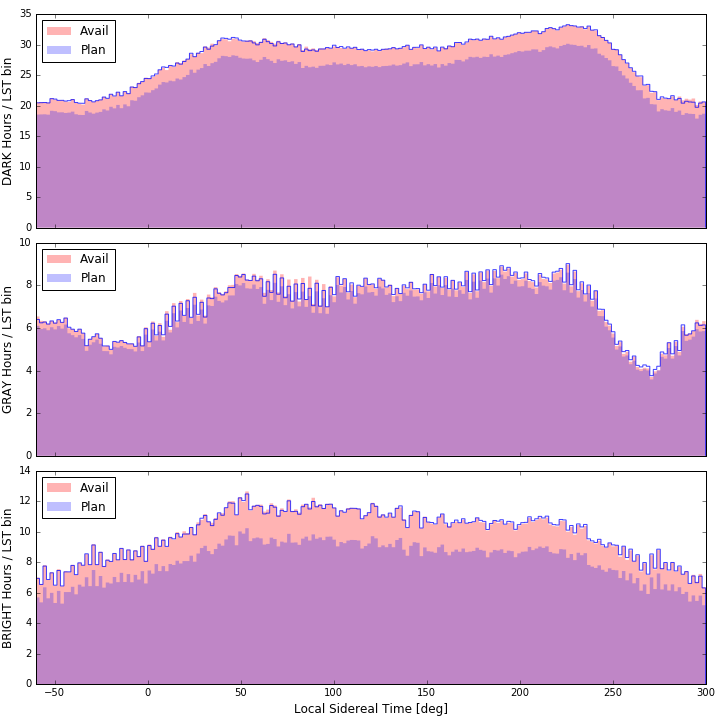
\includegraphics[width=6in]{LST_zero}
\caption{Available (red) and planned (blue) LST usage after optimizing initial HA=0 assignments.  The blue outline histogram shows the planned usage rescaled to the area of the available LST histogram.  The LST axis starts at $-60^\circ$.}
\label{fig:LST_zero}
\end{center}
\end{figure}

\begin{figure}[htb]
\begin{center}
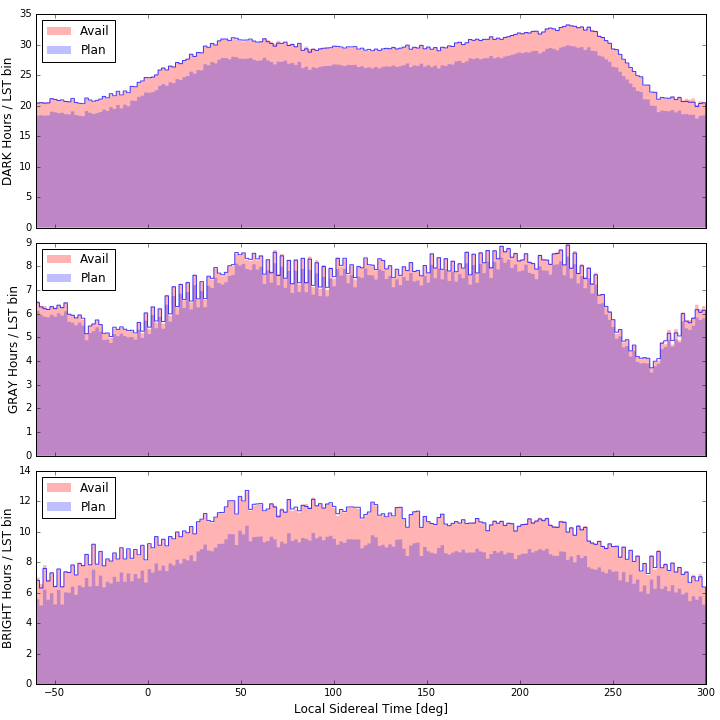
\includegraphics[width=6in]{LST_flat}
\caption{Available (red) and planned (blue) LST usage after optimizing initial HAs obtained with the ``flat'' method.  The blue outline histogram shows the planned usage rescaled to the area of the available LST histogram.  The LST axis starts at $-60^\circ$.}
\label{fig:LST_flat}
\end{center}
\end{figure}

\begin{figure}[htb]
\begin{center}
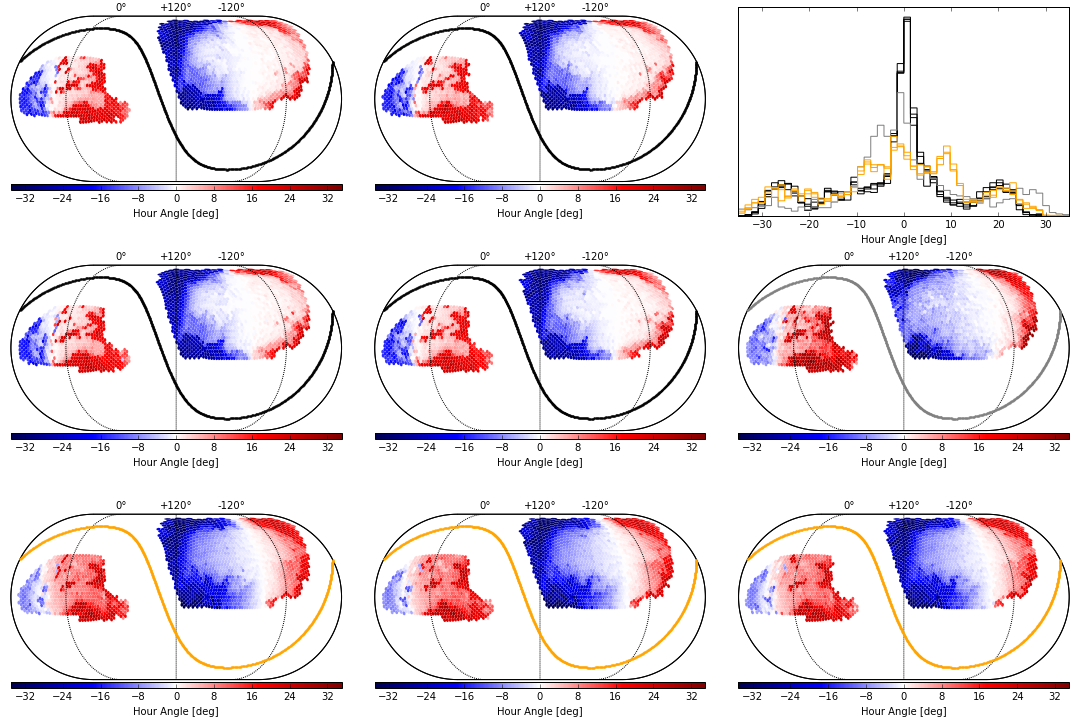
\includegraphics[width=6in]{HA_zero}
\caption{All-sky maps of the tiles in each pass (0-7) color coded by their initial HA assignment after optimizing initial HA=0 assignments.}
\label{fig:HA_zero}
\end{center}
\end{figure}

\begin{figure}[htb]
\begin{center}
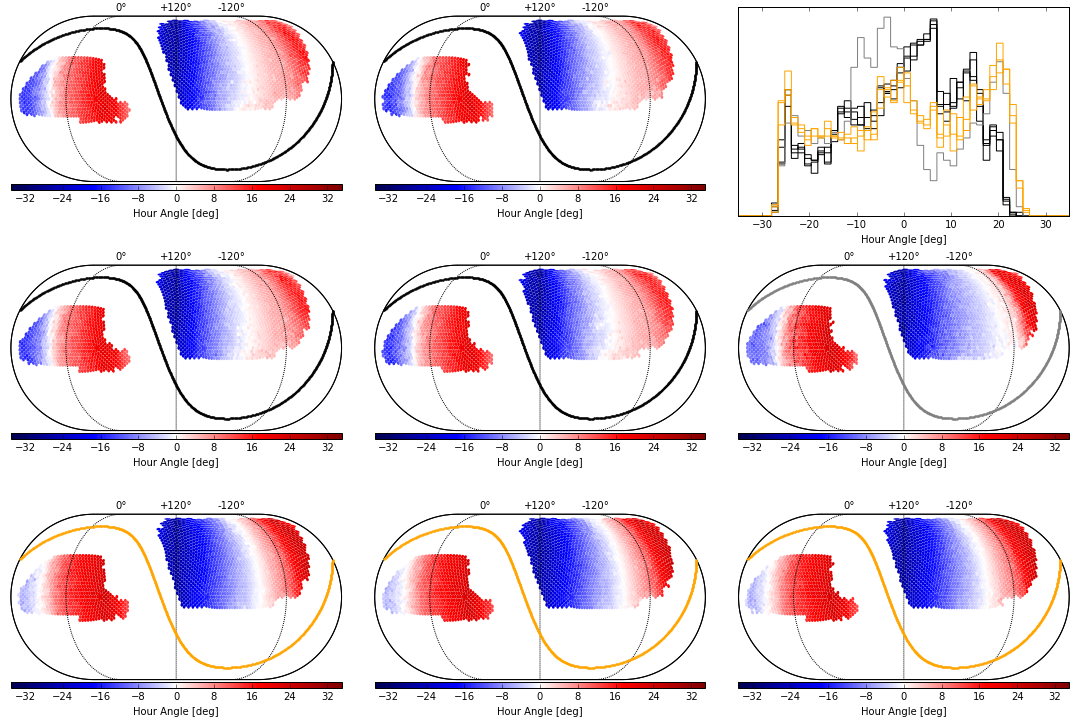
\includegraphics[width=6in]{HA_flat}
\caption{All-sky maps of the tiles in each pass (0-7) color coded by their initial HA assignment after optimizing initial HA=0 assignments.}
\label{fig:HA_flat}
\end{center}
\end{figure}

\begin{table}[htb]
\begin{center}
\begin{tabular}{lcccc}
Program & Available & Planned & Stretch & Margin \\
\hline
DARK   & 5319.0h & 4784.9h & 1.4 & 11.2\% \\
GRAY   & 1357.8h & 1284.4h & 1.5 &  5.7\% \\
BRIGHT & 1899.8h & 1553.0h & 2.0 & 22.3\% \\
\hline
\end{tabular}
\caption{Summary of observing plan for each program based on the observing hour angle assignments obtained with the ``flat'' initialization method.}
\label{tab:summary}
\end{center}
\end{table}

\def\apjl{ApJL} %Astrophysical Journal Letters
\def\aj{AJ} %Astronomical Journal
\def\apj{ApJ} %Astrophysical Journal
\def\pasp{PASP} %Publications of the Astronomical Society of the Pacific
\def\spie{SPIE} %
\def\apjs{ApJS} %Astrophysical Journal Supplement
\def\araa{ARAA} %Annual Review of Astronomy and Astrophysics
\def\aap{A\&A} %Astronomy and Astrophysics
\def\aaps{A\&A~Supl.} %Astronomy and Astrophysics Supplement
\def\nat{Nature} %Nature
\def\nar{New Astron. Rev.} %New Astronomy Review
\def\mnras{MNRAS} %Monthly Notices of the Royal Astronomical Society
\def\jcap{JCAP} %Journal of Cosmology and Astroparticle physics
\def\prd{{Phys.~Rev.~D}}        % Physical Review D
\def\physrep{{Phys.~Reports}} % Physics Reports

\bibliographystyle{unsrt}
\bibliography{design_ha}

\end{document}
